% Copyright 2006 by Till Tantau
%
% This file may be distributed and/or modified
%
% 1. under the LaTeX Project Public License and/or
% 2. under the GNU Free Documentation License.
%
% See the file doc/generic/pgf/licenses/LICENSE for more details.


\section{Calendar Library}
\label{section-calender}

\begin{tikzlibrary}{calendar}
    The library defines the |\calendar| command, which can be used to typeset
    calendars. The command relies on the |\pgfcalendar| command from the
    |pgfcalendar| package, which is loaded automatically.

    The |\calendar| command is quite configurable, allowing you to produce all
    kinds of different calendars.
\end{tikzlibrary}
%
\begin{codeexample}[setup code,hidden]
    \usetikzlibrary{calendar}
\end{codeexample}


\subsection{Calendar Command}

The core command for creating calendars in \tikzname\ is the |\calendar|
command. It is available only inside |{tikzpicture}| environments (similar to,
say, the |\draw| command).

\begin{command}{\calendar \meta{calendar specification}|;|}
    The syntax for this command is similar to commands like |\node| or
    |\matrix|. However, it has its complete own parser and only those commands
    described in the following will be recognized, nothing else. Note,
    furthermore, that a \meta{calendar specification} is not a path
    specification, indeed, no path is created for the calendar.


    \medskip
    \textbf{The specification syntax.}
    The \meta{calendar specification} must be a sequence of elements, each of
    which has one of the following structures:
    %
    \begin{itemize}
        \item |[|\meta{options}|]|

            You provide \meta{options} in square brackets as in
            |[red,draw=none]|. These \meta{options} can be any \tikzname\
            option and they apply to the whole calendar. You can provide this
            element multiple times, the effect accumulates.
        \item |(|\meta{name}|)|

            This has the same effect as saying |[name=|\meta{name}|]|. The
            effect of providing a \meta{name} is explained later. Note already
            that \emph{a calendar is not a node} and the \meta{name} is
            \emph{not the name of a node}.
        \item |at (|\meta{coordinate}|)|

            This has the same effect as saying |[at=(|\meta{coordinate}|)]|.
        \item |if (|\meta{date condition}|)| \meta{options or commands}\opt{|else|\meta{else options or commands}}

            The effect of such an |if| is explained later.
  \end{itemize}

    At the beginning of every calendar, the following style is used:
    %
    \begin{stylekey}{/tikz/every calendar (initially \normalfont empty)}
        This style is used with every calendar.
    \end{stylekey}


    \medskip
    \textbf{The date range.}
    The overall effect of the |\calendar| command is to execute code for each
    day of a range of dates. This range of dates is set using the following
    option:
    %
    \begin{key}{/tikz/dates=\meta{start date}| to |\meta{end date}}
        This option specifies the date range. Both the start and end date are
        specified as described on page~\pageref{calendar-date-format}. In
        short: You can provide ISO-format type dates like |2006-01-02|, you can
        replace the day of month by |last| to refer to the last day of a month
        (so |2006-02-last| is the same as |2006-02-28|), and you can add a plus
        sign followed by a number to specify an offset (so |2006-01-01+-1| is
        the same as |2005-12-31|).
    \end{key}
    %
    It will be useful to fix two pieces of terminology for the following
    descriptions: The |\calendar| command iterates over the dates in the range.
    The \emph{current date} refers to the current date the command is
    processing as it iterates over the dates. For each current date code is
    executed, which will be called the \emph{current date code}. The current
    date code consists of different parts, to be detailed later.

    The central part of the current date code is the execution of the code
    |\tikzdaycode|. By default, this code simply produces a node whose text is
    set to the day of month. This means that unless further action is taken,
    all days of a calendar will be put on top of each other! To avoid this, you
    must modify the current date code to shift days around appropriately.
    Predefined arrangements like |day list downward| or |week list| do this for
    you, but you can define arrangements yourself. Since defining an
    arrangement is a bit tricky, it is explained only later on. For the time
    being, let us use a predefined arrangement to produce our first calendar:
    %
\begin{codeexample}[]
\tikz \calendar[dates=2000-01-01 to 2000-01-31,week list];
\end{codeexample}


    \medskip
    \textbf{Changing the spacing.}
    In the above calendar, the spacing between the days is determined by
    numerous options. Most arrangements do not use all of these options, but
    only those that apply naturally.
    %
    \begin{key}{/tikz/day xshift=\meta{dimension} (initially 3.5ex)}
        Specifies the horizontal shift between days. This is not the gap
        between days, but the shift between the anchors of their nodes.
        %
\begin{codeexample}[]
\tikz \calendar[dates=2000-01-01 to 2000-01-31,week list,day xshift=3ex];
\end{codeexample}
    \end{key}
    %
    \begin{key}{/tikz/day yshift=\meta{dimension} (initially 3ex)}
        Specifies the vertical shift between days. Again, this is the shift
        between the anchors of their nodes.
        %
\begin{codeexample}[]
\tikz \calendar[dates=2000-01-01 to 2000-01-31,week list,day yshift=2ex];
\end{codeexample}
    \end{key}
    %
    \begin{key}{/tikz/month xshift=\meta{dimension}}
        Specifies an additional  horizontal shift between different months.
    \end{key}
    %
    \begin{key}{/tikz/month yshift=\meta{dimension}}
        Specifies an additional  vertical shift between different months.
        %
\begin{codeexample}[]
\tikz \calendar[dates=2000-01-01 to 2000-02-last,week list,
                month yshift=0pt];
\end{codeexample}
        %
\begin{codeexample}[]
\tikz \calendar[dates=2000-01-01 to 2000-02-last,week list,
                month yshift=1cm];
\end{codeexample}
    \end{key}


    \medskip
    \textbf{Changing the position of the calendar.}
    The calendar is placed in such a way that, normally, the anchor of the
    first day label is at the origin. This can be changed by using the |at|
    option. When you say |at={(1,1)}|, this anchor of the first day will lie at
    coordinate $(1,1)$.

    In general, arrangements will not always place the anchor of the first day
    at the origin. Sometimes, additional spacing rules get in the way. There
    are different ways of addressing this problem: First, you can just ignore
    it. Since calendars are often placed in their own |{tikzpicture}| and since
    their size if computed automatically, the exact position of the origin
    often does not matter at all. Second, you can put the calendar inside a
    node as in |...node {\tikz \calendar...}|. This allows you to position the
    node in the normal ways using the node's anchors. Third, you can be very
    clever and use a single-cell matrix. The advantage is that a matrix allows
    you to provide any anchor of any node inside the matrix as an anchor for
    the whole matrix. For example, the following calendar is placed in such a
    way the center of 2000-01-20 lies on the position $(2,2)$:
    %
\begin{codeexample}[]
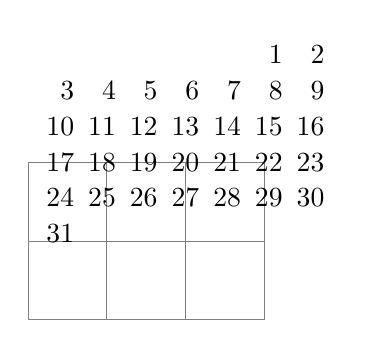
\begin{tikzpicture}
  \draw[help lines] (0,0) grid (3,2);
  \matrix [anchor=cal-2000-01-20.center] at (2,2)
  { \calendar(cal)[dates=2000-01-01 to 2000-01-31,week list]; \\};
\end{tikzpicture}
\end{codeexample}
    %
    Unfortunately, the matrix-base positions, which is the cleanest way, isn't
    as portable as the other approaches (it currently does not work with the
    \textsc{svg} backend for instance).


    \medskip
    \textbf{Changing the appearance of days.}
    As mentioned before, each day in the above calendar is produced by an
    execution of the |\tikzdaycode|. Each time this code is executed, the
    coordinate system will have been set up appropriately to place the day of
    the month correctly. You can change both the code and its appearance using
    the following options.
    %
    \begin{key}{/tikz/day code=\meta{code} (initially \normalfont see below)}
        This option allows you to change the code that is executed for each
        day. The default is to create a node with an appropriate name, but you
        can change this:
        %
\begin{codeexample}[]
\tikz \calendar[dates=2000-01-01 to 2000-01-31,week list,
                day code={\fill[blue] (0,0) circle (2pt);}];
\end{codeexample}
        %
        The default code is the following:
        %
\begin{codeexample}[code only]
\node[name=\pgfcalendarsuggestedname,every day]{\tikzdaytext};
\end{codeexample}
        %
        The first part causes the day nodes to be accessible via the following
        names: If \meta{name} is the name given to the calendar via a |name=|
        option or via the specification element |(|\meta{name}|)|, then
        |\pgfcalendarsuggestedname| will expand to \meta{name}|-|\meta{date},
        where \meta{date} is the date of the day that is currently being
        processed in ISO format.

        For example, if January 1, 2006 is being processed and the calendar has
        been named |mycal|, then the node containing the |1| for this date will
        be names |mycal-2006-01-01|. You can later reference this node.
        %
\begin{codeexample}[]
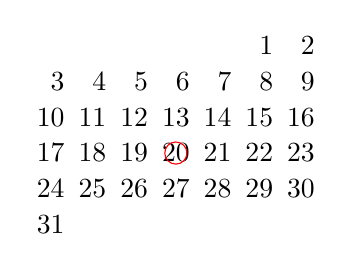
\begin{tikzpicture}
  \calendar (mycal) [dates=2000-01-01 to 2000-01-31,week list];

  \draw[red] (mycal-2000-01-20) circle (4pt);
\end{tikzpicture}
\end{codeexample}
    \end{key}

    \begin{key}{/tikz/day text=\meta{text}}
        This option changes the setting of the |\tikzdaytext|. By default, this
        macro simply yields the current day of month, but you can change it
        arbitrarily. Here is a silly example:
        %
\begin{codeexample}[]
\tikz \calendar[dates=2000-01-01 to 2000-01-31,week list,
                day text=x];
\end{codeexample}
        %
        More useful examples are based on using the |\%| command. This command
        is redefined inside a |\pgfcalendar| to mean the same as
        |\pgfcalendarshorthand|. (The original meaning of |\%| is lost inside
        the calendar, you need to save if before the calendar if you really
        need it.)

        The |\%| inserts the current day/month/year/day of week in a certain
        format into the text. The first letter following the |\%| selects the
        type (permissible values are |d|, |m|, |y|, |w|), the second letter
        specifies how the value should be displayed (|-| means numerically, |=|
        means numerically with leading space, |0| means numerically with
        leading zeros, |t| means textual, and |.| means textual, abbreviated).
        For example |\%d0| gives the day with a leading zero (for more details
        see the description of |\pgfcalendarshorthand| on
        page~\pageref{pgfcalendarshorthand}).

        Let us redefine the |day text| so that it yields the day with a leading
        zero:
        %
\begin{codeexample}[leave comments]
\tikz \calendar[dates=2000-01-01 to 2000-01-31,week list,
                day text=\%d0];
\end{codeexample}
    \end{key}

    \begin{key}{/tikz/every day (initially anchor=base east)}
        This style is executed by the default node code for each day. The
        |every day| style is useful for changing the way days look. For
        example, let us make all days red:
        %
\begin{codeexample}[leave comments]
\tikz[every day/.style=red]
  \calendar[dates=2000-01-01 to 2000-01-31,week list];
\end{codeexample}
    \end{key}


    \medskip
    \textbf{Changing the appearance of month and year labels.}
    In addition to the days of a calendar, labels for the months and even years
    (for really long calendars) can be added. These labels are only added once
    per month or year and this is not done by default. Rather, special styles
    starting with |month label| place these labels and make them visible:
    %
\begin{codeexample}[]
\tikz \calendar[dates=2000-01-01 to 2000-02-last,week list,
                month label above centered];
\end{codeexample}

    The following options change the appearance of the month and year label:
    %
    \begin{key}{/tikz/month code=\meta{code} (initially \normalfont see below)}
        This option allows you to specify what the macro |\tikzmonthcode|
        should expand to.

        By default, the |\tikzmonthcode| it is set to
        %
\begin{codeexample}[code only]
\node[every month]{\tikzmonthtext};
\end{codeexample}
        %
        Note that this node is not named by default.
    \end{key}

    \begin{key}{/tikz/month text=\meta{text}}
        This option allows you to change the macro |\tikzmonthtext|. By
        default, the month text is a long textual presentation of the current
        month being typeset.
        %
\begin{codeexample}[leave comments]
\tikz \calendar[dates=2000-01-01 to 2000-01-31,week list,
                month label above centered,
                month text=\textcolor{red}{\%mt} \%y-];
\end{codeexample}
    \end{key}

    \begin{stylekey}{/tikz/every month (initially \normalfont empty)}
        This style can be used to change the appearance of month labels.
    \end{stylekey}

    \begin{key}{/tikz/year code=\meta{code}}
        Works like |month code|, only for years.
    \end{key}

    \begin{key}{/tikz/year text=\meta{text}}
        Works like |month text|, only for years.
    \end{key}


    \begin{key}{/tikz/every year}
        Works like |every month|, only for years.
    \end{key}


    \medskip
    \textbf{Date ifs.}
    Much of the power of the |\calendar| command comes from the use of
    conditionals. There are two equivalent way of specifying such a
    conditional. First, you can add the text
    |if (|\meta{conditions}|) |\meta{code or options} to your \meta{calendar
    specification}, possibly followed by |else|\meta{else code or options}. You
    can have multiple such conditionals (but you cannot nest them in this
    simple manner). The second way is to use the following option:
    %
    \begin{key}{/tikz/if=|(|\meta{conditions}|)|\meta{code or options}\opt{|else|\meta{else code or options}}}
        This option has the same effect as giving a corresponding if in the
        \meta{calendar specification}. The option is mostly useful for use in
        the |every calendar| style, where you cannot provide if conditionals
        otherwise.
    \end{key}
    %
    Now, regardless of how you specify a conditional, it has the following
    effect (individually and independently for each date in the calendar):
    %
    \begin{enumerate}
        \item It is checked whether the current date is one of the
            possibilities listed in \meta{conditions}. An example of such a
            condition is |Sunday|. Thus, when you write
            |if (Saturday,Sunday) {foo}|, then |foo| will be executed for every
            day in the calendar that is a Saturday \emph{or} a Sunday.

            The command |\ifdate| and, thereby, |\pgfcalendarifdate| are used
            to evaluate the \meta{conditions}, see
            page~\pageref{pgfcalendarifdate} for a complete list of possible
            tests. The most useful tests are: Tests like |Monday| and so on,
            |workday| for the days Monday to Friday, |weekend| for Saturday and
            Sunday, |equals| for testing whether the current date equals a
            given date, |at least| and |at least| for comparing the current
            date with a given date.
        \item If the date passes the check, the \meta{code or options} is
            evaluated in a manner to be described in a moment; if the date
            fails, the \meta{else code or options} is evaluated, if present.

            The \meta{code or options} can either be some code. This is
            indicated by surrounding the code with curly braces. It can also be
            a list of \tikzname\ options. This is indicated by surrounding the
            options with square brackets. For example in the date test
            |if (Sunday) {\draw...} else {\fill...}| there are two pieces of
            code involved. By comparison, |if (Sunday) [red] else [green]|
            involves two options.

            If \meta{code or options} is code, it is simply executed (for the
            current day). If it is a list of options, these options are passed
            to a scope surrounding the current date.
    \end{enumerate}
    %
    Let us now have a look at some examples. First, we use a conditional to
    make all Sundays red.
    %
\begin{codeexample}[]
\tikz
  \calendar
    [dates=2000-01-01 to 2000-01-31,week list]
    if (Sunday) [red];
\end{codeexample}
    %
    Next, let us do something on a specific date:
    %
\begin{codeexample}[]
\tikz
  \calendar
    [dates=2000-01-01 to 2000-01-31,week list]
    if (Sunday)            [red]
    if (equals=2000-01-20) {\draw (0,0) circle (8pt);};
\end{codeexample}
    %
    You might wonder why the circle seems to be ``off'' the date. Actually, it
    is centered on the date, it is just that the date label uses the
    |base east| anchor, which shifts the label up and right. To overcome this
    problem we can change the anchor:
    %
\begin{codeexample}[]
\tikz [every day/.style={anchor=mid}]
  \calendar
    [dates=2000-01-01 to 2000-01-31,week list]
    if (Sunday)            [red]
    if (equals=2000-01-20) {\draw (0,0) circle (8pt);};
\end{codeexample}
    %
    However, the single day dates are now no longer aligned correctly. For
    this, we can change the day text to |\%d=|, which adds a space at the
    beginning of single day text.

    In the following, more technical information is covered. Most readers may
    wish to skip it.

    \medskip
    \textbf{The current date code.}
    As mentioned earlier, for each date in the calendar the current date code
    is executed. It is the job of this code to shift around date nodes, to
    render the date nodes, to draw the month labels and to do all other stuff
    that is necessary to draw a calendar.

    The current date code consists of the following parts, in this order:
    %
    \begin{enumerate}
        \item The before-scope code.
        \item A scope is opened.
        \item The at-begin-scope code.
        \item All date-ifs from the \meta{calendar specification} are executed.
        \item The at-end-scope code.
        \item The scope is closed.
        \item The after-scope code.
    \end{enumerate}
    %
    All of the codes mentioned above can be changed using appropriate options,
    see below. In case you wonder why so many are needed, the reason is that
    the current date code as a whole is not surrounded by a scope or \TeX\
    group. This means that code executed in the before-scope code and in the
    after-scope code has an effect on all following days. For example, if the
    after-scope code modifies the transformation matrix by shifting everything
    downward, all following days will be shifted downward. If each day does
    this, you get a list of days, one below the other.

    However, you do not always want code to have an effect on everything that
    follows. For instance, if a day has the date-if |if (Sunday) [red]|, we
    only want this Sunday to red, not all following days also. Similarly,
    sometimes it is easier to compute the position of a day relative to a fixed
    origin and we do not want any modifications of the transformation matrix to
    have an effect outside the scope.

    By cleverly adjusting the different codes, all sorts of different day
    arrangements are possible.

    \begin{key}{/tikz/execute before day scope=\meta{code}}
        The \meta{code} is executed before everything else for each date.
        Multiple calls of this option have an accumulative effect. Thus, if you
        use this option twice, the code from the first use is used first for
        each day, followed by the code given the second time.
    \end{key}
    %
    \begin{key}{/tikz/execute at begin day scope=\meta{code}}
        This code is execute before everything else inside the scope of the
        current date. Again, the effect is accumulative.
    \end{key}
    %
    \begin{key}{/tikz/execute at end day scope=\meta{code}}
        This code is executed just before the day scope is closed. The effect
        is also accumulative, however, in reverse order. This is useful to
        pair, say, |\scope| and |\endscope| commands in at-begin- and
        at-end-code.
    \end{key}
    %
    \begin{key}{/tikz/execute after day scope=\meta{code}}
        This is executed at the very end of the current date, outside the
        scope. The accumulation is also in reverse.
    \end{key}
\end{command}

In the rest of the following subsections we have a look at how the different
scope codes can be used to create different calendar arrangements.


\subsubsection{Creating a Simple List of Days}

We start with a list of the days of the calendar, one day below the other. For
this, we simply shift the coordinate system downward at the end of the code for
each day. This shift must be \emph{outside} the day scope as we want day shifts
to accumulate. Thus, we use the following code:
%
\begin{codeexample}[]
\tikz
  \calendar [dates=2000-01-01 to 2000-01-08,
             execute after day scope=
               {\pgftransformyshift{-1em}}];
\end{codeexample}
%
Clearly, we can use this approach to create day lists going up, down, right,
left, or even diagonally.


\subsubsection{Adding a Month Label}

We now want to add a month label to the left of the beginning of each month.
The idea is to do two things:
%
\begin{enumerate}
    \item We add code that is executed only on the first of each month.
    \item The code is executed before the actual day is rendered. This ensures
        that options applying to the days do not affect the month rendering.
\end{enumerate}
%
We have two options where we should add the month code: Either we add it at the
beginning of the day scope or before. Either will work fine, but it might be
safer to put the code inside the scope to ensure that settings to not
inadvertently ``leak outside''.
%
\begin{codeexample}[]
\tikz
  \calendar
    [dates=2000-01-01 to 2000-01-08,
     execute after day scope={\pgftransformyshift{-1em}},
     execute at begin day scope=
       {\ifdate{day of month=1}{\tikzmonthcode}{}},
     every month/.append style={anchor=base east,xshift=-2em}];
\end{codeexample}

In the above code we used the |\ifdate|\marg{condition}\marg{then
code}\marg{else code} command, which is described on page~\pageref{ifdate} in
detail and which has much the same effect as
|if (|\meta{condition}|)|\marg{then code}| else |\marg{else code}, but works in
normal code.


\subsubsection{Creating a Week List Arrangement}

Let us now address a more complicated arrangement: A week list. In this
arrangement there is line for each week. The horizontal placement of the days
is thus that all Mondays lie below each other, likewise for all Tuesdays, and
so on.

In order to typeset this arrangement, we can use the following approach: The
origin of the coordinate system rests at the anchor for the Monday of each
week. That means that at the end of each week the origin is moved downward one
line. On all other days, the origin at the end of the day code is the same as
at the beginning. To position each day correctly, we use code inside and at the
beginning of the day scope to horizontally shift the day according to its day
of week.
%
\begin{codeexample}[]
\tikz
  \calendar
    [dates=2000-01-01 to 2000-01-20,
     % each day is shifted right according to the day of week
     execute at begin day scope=
       {\pgftransformxshift{\pgfcalendarcurrentweekday em}},
     % after each week, the origin is shifted downward:
     execute after day scope=
       {\ifdate{Sunday}{\pgftransformyshift{-1em}}{}}];
\end{codeexample}


\subsubsection{Creating a Month List Arrangement}

For another example, let us create an arrangement that contains one line for
each month. This is easy enough to do as for weeks, unless we add the following
requirement: Again, we want all days in a column to have the same day of week.
Since months start on different days of week, this means that each row has to
have an individual offset.

One possible way is to use the following approach: After each month (or at the
beginning of each month) we advance the vertical position of the offset by one
line. For horizontal placement, inside the day scope we locally shift the day
by its day of month. Furthermore, we must additionally shift the day to ensure
that the first day of the month lies on the correct day of week column. For
this, we remember this day of week the first time we see it.
%
\begin{codeexample}[]
\newcount\mycount
\tikz
  \calendar
    [dates=2000-01-01 to 2000-02-last,
     execute before day scope=
     {
       \ifdate{day of month=1} {
         % Remember the weekday of first day of month
         \mycount=\pgfcalendarcurrentweekday
         % Shift downward
         \pgftransformyshift{-1em}
       }{}
     },
     execute at begin day scope=
     {
       % each day is shifted right according to the day of month
       \pgftransformxshift{\pgfcalendarcurrentday em}
       % and additionally according to the weekday of the first
       \pgftransformxshift{\the\mycount em}
     }];
\end{codeexample}


\subsection{Arrangements}

An \emph{arrangement} specifies how the days of calendar are arranged on the
page. The calendar library defines a number of predefined arrangements.

We start with arrangements in which the days are listed in a long line.

\begin{stylekey}{/tikz/day list downward}
    This style causes the days of a month to be typeset one below the other.
    The shift between days is given by |day yshift|. Between month an
    additional shift of |month yshift| is added.
    %
\begin{codeexample}[]
\tikz
  \calendar [dates=2000-01-28 to 2000-02-03,
             day list downward,month yshift=1em];
\end{codeexample}
    %
\end{stylekey}

\begin{stylekey}{/tikz/day list upward}
    Works as above, only the list grows upward instead of downward.
    %
\begin{codeexample}[]
\tikz
  \calendar [dates=2000-01-28 to 2000-02-03,
             day list upward,month yshift=1em];
\end{codeexample}
    %
\end{stylekey}

\begin{stylekey}{/tikz/day list right}
    This style also works as before, but the list of days grows to the right.
    Instead of |day yshift| and |month yshift|, the values of |day xshift| and
    |month xshift| are used.
    %
\begin{codeexample}[]
\tikz
  \calendar [dates=2000-01-28 to 2000-02-03,
             day list right,month xshift=1em];
\end{codeexample}
    %
\end{stylekey}

\begin{stylekey}{/tikz/day list left}
    As above, but the list grows left.
\end{stylekey}

The next arrangement lists days by the week.

\begin{stylekey}{/tikz/week list}
    This style creates one row for each week in the range. The value of
    |day xshift| is used for the distance between days in each week row, the
    value of |day yshift| is used for the distance between rows. In both cases,
    ``distance'' refers to the distance between the anchors of the nodes of the
    days (or, more generally, the distance between the origins of the little
    pictures created for each day).

    The days inside each week are shifted such that Monday is always at the
    first position (to change this, you need to copy and then modify the code
    appropriately). If the date range does not start on a Monday, the first
    line will not start in the first column, but rather in the column
    appropriate for the first date in the range.

    At the beginning of each month (except for the first month in the range) an
    additional vertical space of |month yshift| is added. If this is set to
    |0pt| you get a continuous list of days.
    %
\begin{codeexample}[]
\tikz
  \calendar [dates=2000-01-01 to 2000-02-last,week list];
\end{codeexample}
    %
\begin{codeexample}[]
\tikz
  \calendar [dates=2000-01-01 to 2000-02-last,week list,
             month yshift=0pt];
\end{codeexample}
    %
\end{stylekey}

The following arrangement gives a very compact view of a whole year.
%
\begin{stylekey}{/tikz/month list}
    In this arrangement there is a row for each month. As for the |week list|,
    the |day xshift| is used for the horizontal distance. For the vertical
    shift, |month yshift| is used.

    In each row, all days of the month are listed alongside each other.
    However, it is once more ensured that days in each column lie on the same
    day of week. Thus, the very first column contains only Mondays. If a month
    does not start with a Monday, its days are shifted to the right such that
    the days lie on the correct columns.
    %
\begin{codeexample}[]
\sffamily\scriptsize
\tikz
  \calendar [dates=2000-01-01 to 2000-12-31,
             month list,month label left,month yshift=1.25em]
            if (Sunday) [black!50];
\end{codeexample}
    %
\end{stylekey}


\subsection{Month Labels}

For many calendars you may wish to add a label to each month. We have already
covered how month nodes are created and rendered in the description of the
|\calendar| command: use |month text|, |every month|, and also |month code| (if
necessary) to change the appearance of the month labels.

What we have not yet covered is where these labels are placed. By default, they
are not placed at all as there is no good ``default position'' for them.
Instead, you can use one of the following options to specify a position for the
labels:
%
\begin{stylekey}{/tikz/month label left}
    Places the month label to the left of the first day of the month. (For
    |week list| and |month list| where a month does not start on a Monday, the
    position is chosen ``as if'' the month had started on a Monday --  which is
    usually exactly what you want.)
    %
\begin{codeexample}[]
\tikz
  \calendar [dates=2000-01-28 to 2000-02-03,
             day list downward,month yshift=1em,
             month label left];
\end{codeexample}
    %
\end{stylekey}

\begin{stylekey}{/tikz/month label left vertical}
    This style works like the above style, only the label is rotated
    counterclockwise by 90 degrees.
    %
\begin{codeexample}[]
\tikz
  \calendar [dates=2000-01-28 to 2000-02-03,
             day list downward,month yshift=1em,
             month label left vertical];
\end{codeexample}
    %
\end{stylekey}

\begin{stylekey}{/tikz/month label right}
    This style places the month label to the right of the row in which the
    first day of the month lies. This means that for a day list the label is to
    the right of the first day, for a week list it is to the right of the first
    week, and for a month list it is to the right of the whole month.
    %
\begin{codeexample}[]
\tikz
  \calendar [dates=2000-01-28 to 2000-02-03,
             day list downward,month yshift=1em,
             month label right];
\end{codeexample}
    %
\end{stylekey}

\begin{stylekey}{/tikz/month label right vertical}
    Works as above, only the label is rotated clockwise by 90 degrees.
    %
\begin{codeexample}[]
\tikz
  \calendar [dates=2000-01-28 to 2000-02-03,
             day list downward,month yshift=1em,
             month label right vertical];
\end{codeexample}
    %
\end{stylekey}

\begin{stylekey}{/tikz/month label above left}
    This style places the month label above of the row of the first day,
    flushed left to the leftmost column. The amount by which the label is
    raised is fixed to |1.25em|; use the |yshift| option with the month node to
    modify this.
    %
\begin{codeexample}[]
\tikz
  \calendar [dates=2000-01-28 to 2000-02-03,
             day list right,month xshift=1em,
             month label above left];
\end{codeexample}
    %
\begin{codeexample}[]
\tikz
  \calendar [dates=2000-01-20 to 2000-02-10,
             week list,month label above left];
\end{codeexample}
    %
\end{stylekey}

\begin{stylekey}{/tikz/month label above centered}
    Works as above, only the label is centered above the row containing the
    first day.
    %
\begin{codeexample}[]
\tikz
  \calendar [dates=2000-02-01 to 2000-02-last,
             day list right,month label above centered];
\end{codeexample}
    %
\begin{codeexample}[]
\tikz
  \calendar [dates=2000-01-20 to 2000-02-10,
             week list,month label above centered];
\end{codeexample}
    %
\end{stylekey}

\begin{stylekey}{/tikz/month label above right}
    Works as above, but flushed right
    %
\begin{codeexample}[]
\tikz
  \calendar [dates=2000-01-20 to 2000-02-10,
             week list,month label above right];
\end{codeexample}
    %
\end{stylekey}

\begin{stylekey}{/tikz/month label below left}
    Works like |month label above left|, only the label is placed below the
    row. This placement is not really useful with the |week list| arrangement,
    but rather with the |day list right| or |month list| arrangement.
    %
\begin{codeexample}[]
\tikz
  \calendar [dates=2000-02-01 to 2000-02-last,
             day list right,month label below left];
\end{codeexample}
    %
\end{stylekey}

\begin{stylekey}{/tikz/month label below centered}
    Works like |month label above centered|, only below.
    %
\begin{codeexample}[]
\tikz
  \calendar [dates=2000-02-01 to 2000-02-last,
             day list right,month label below centered];
\end{codeexample}
    %
\end{stylekey}


\subsection{Examples}

In the following, some example calendars are shown that come either from real
applications or are just nice to look at.

Let us start with a year-2100-countdown, in which we cross out dates as we
approach the big celebration. For this, we set the shape to |strike out| for
these dates.
%
\begin{codeexample}[leave comments]
\begin{tikzpicture}
  \calendar
  [
    dates=2099-12-01 to 2100-01-last,
    week list,inner sep=2pt,month label above centered,
    month text=\%mt \%y0
  ]
  if (at most=2099-12-29) [nodes={strike out,draw}]
  if (weekend)            [black!50,nodes={draw=none}]
  ;
\end{tikzpicture}
\end{codeexample}

The next calendar shows a deadline, which is 10 days in the future from the
current date. The last three days before the deadline are in red, because we
really should be done by then. All days on which we can no longer work on the
project are crossed out.
%
\begin{codeexample}[leave comments]
\begin{tikzpicture}
  \calendar
  [
    dates=\year-\month-\day+-25 to \year-\month-\day+25,
    week list,inner sep=2pt,month label above centered,
    month text=\textit{\%mt \%y0}
  ]
  if (at least=\year-\month-\day) {}
    else [nodes={strike out,draw}]
  if (at most=\year-\month-\day+7)
    [green!50!black]
  if (between=\year-\month-\day+8 and \year-\month-\day+10)
    [red]
  if (Sunday)
    [gray,nodes={draw=none}]
  ;
\end{tikzpicture}
\end{codeexample}

The following example is a futuristic calendar that is all about circles:
%
\begin{codeexample}[]
\sffamily

\colorlet{winter}{blue}
\colorlet{spring}{green!60!black}
\colorlet{summer}{orange}
\colorlet{fall}{red}

% A counter, since TikZ is not clever enough (yet) to handle
% arbitrary angle systems.
\newcount\mycount

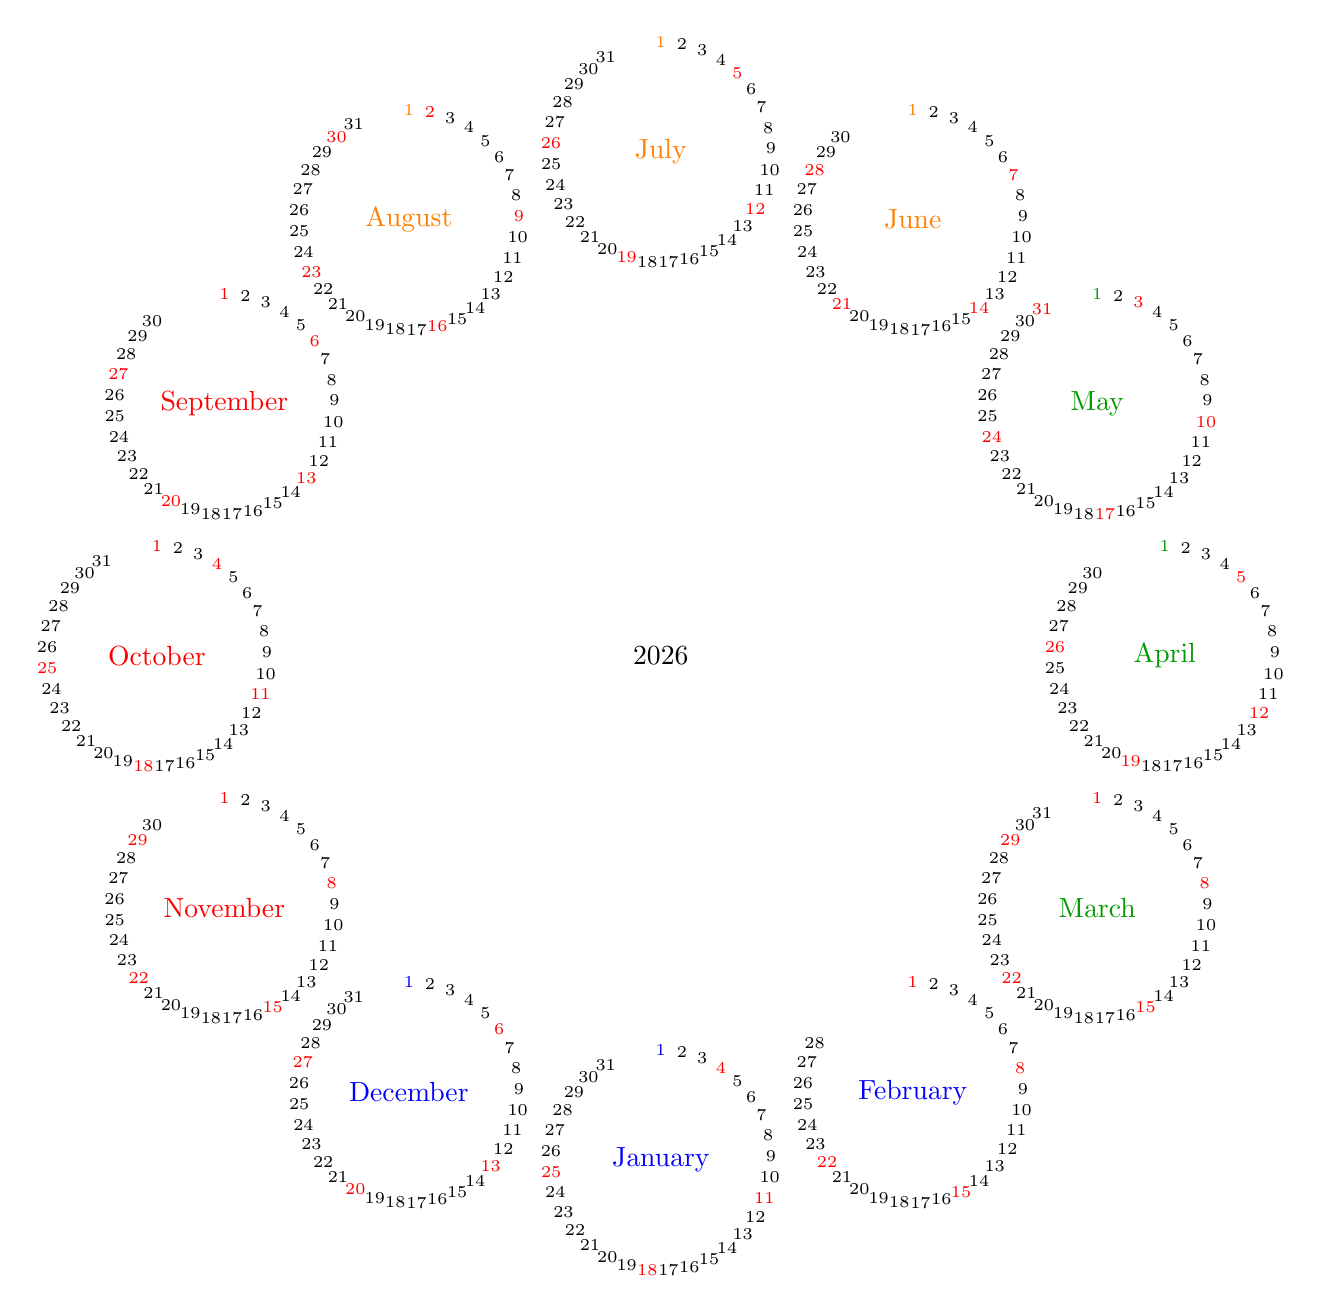
\begin{tikzpicture}
  [transform shape,
   every day/.style={anchor=mid,font=\fontsize{6}{6}\selectfont}]
  \node{\normalsize\the\year};
  \foreach \month/\monthcolor in
    {1/winter,2/winter,3/spring,4/spring,5/spring,6/summer,
     7/summer,8/summer,9/fall,10/fall,11/fall,12/winter}
  {
    % Compute angle:
    \mycount=\month
    \advance\mycount by -1
    \multiply\mycount by 30
    \advance\mycount by -90

    % The actual calendar
    \calendar at (\the\mycount:6.4cm)
    [
      dates=\the\year-\month-01 to \the\year-\month-last,
    ]
    if (day of month=1) {\color{\monthcolor}\tikzmonthcode}
    if (Sunday) [red]
    if (all)
    {
      % Again, compute angle
      \mycount=1
      \advance\mycount by -\pgfcalendarcurrentday
      \multiply\mycount by 11
      \advance\mycount by 90
      \pgftransformshift{\pgfpointpolar{\mycount}{1.4cm}}
    };
  }
\end{tikzpicture}
\end{codeexample}

Next, let's us have a whole year in a tight column:
%
\begin{codeexample}[leave comments]
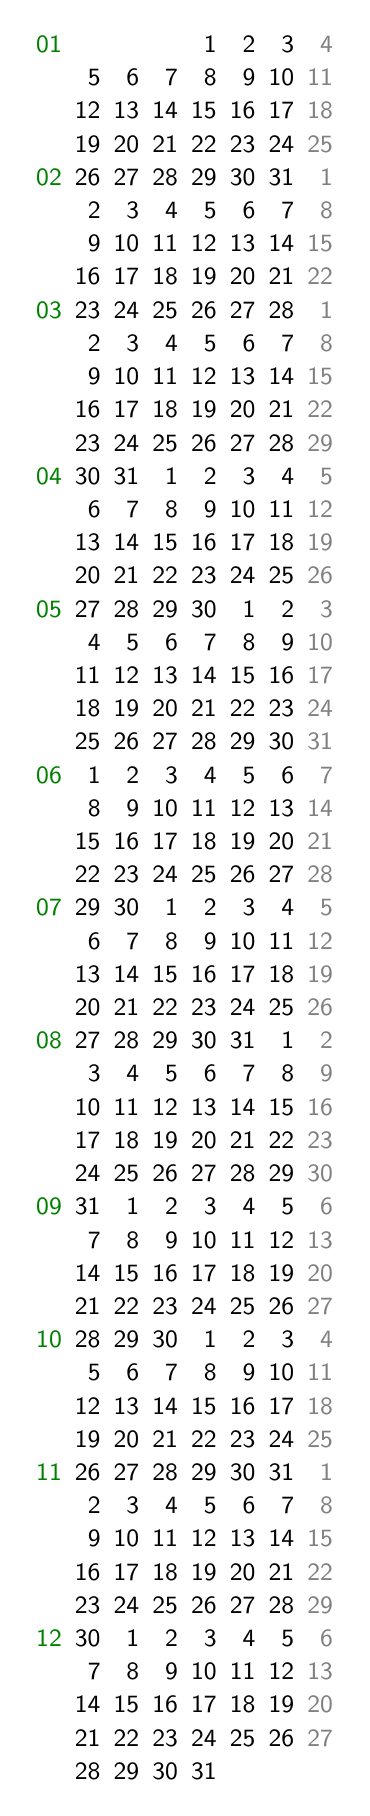
\begin{tikzpicture}
  \small\sffamily
  \colorlet{darkgreen}{green!50!black}
  \calendar[dates=\year-01-01 to \year-12-31,week list,
            month label left,month yshift=0pt,
            month text=\textcolor{darkgreen}{\%m0}]
           if (Sunday) [black!50];
\end{tikzpicture}
\end{codeexample}


%%% Local Variables:
%%% mode: latex
%%% TeX-master: "pgfmanual-pdftex-version"
%%% End:
